%-------------------------------------------------------------------------------
% LATEX TEMPLATE PRESENTATIE
%-------------------------------------------------------------------------------
% Dit template is voor gebruik door studenten van de de bacheloropleiding 
% Informatica van de Universiteit van Amsterdam.
% Voor informatie over presenteren, zie 
%                               https://practicumav.nl/presenteren/index.html
%
%-------------------------------------------------------------------------------
%	PACKAGES EN CONFIGURATIE
%-------------------------------------------------------------------------------
% Gebruik de optie "sidebar" voor toevoeging van een sidebar met inhoudsopgave
% en de optie "dyslexic" voor gebruik van het OpenDyslexic-lettertype
\documentclass[aspectratio=169,sidebar,dyslexic]{uva-inf-presentation}
\usepackage[dutch]{babel}

% Vul hieronder de gevraagde gegevens in, 
% meerdere auteurs en UvAnetID's gescheiden door een puntkomma 
\title{Red-Black Tree} 
\authors{Marouan Bellari; Boris Vukajlovic}
\uvanetids{14675218; UvAnetID student 2}
\course{Academische Vaardigheden}
\tutor{}
\docent{Kas Visser} 
\group{}
\programme{Informatica}

\begin{document}
%-------------------------------------------------------------------------------
%	AUTOMATISCHE SLIDES
%-------------------------------------------------------------------------------
\begin{titelframe}
\titlepage
\end{titelframe}

\begin{titelframe}
\frametitle{Inhoudsopgave}
\tableofcontents
\end{titelframe}

%-------------------------------------------------------------------------------
%	PRESENTATIE SLIDES
%-------------------------------------------------------------------------------
\subsection{(1) Waarom een Red-Black tree?}
\subsection{(2) Hoe werkt een Red-Black tree?}
\subsection{(3) Voorbeeld van een gebroken case}
\subsection{(4) Red-Black tree implementatie}

\begin{frame}
\frametitle{(1) Waarom een Red-Black tree?}
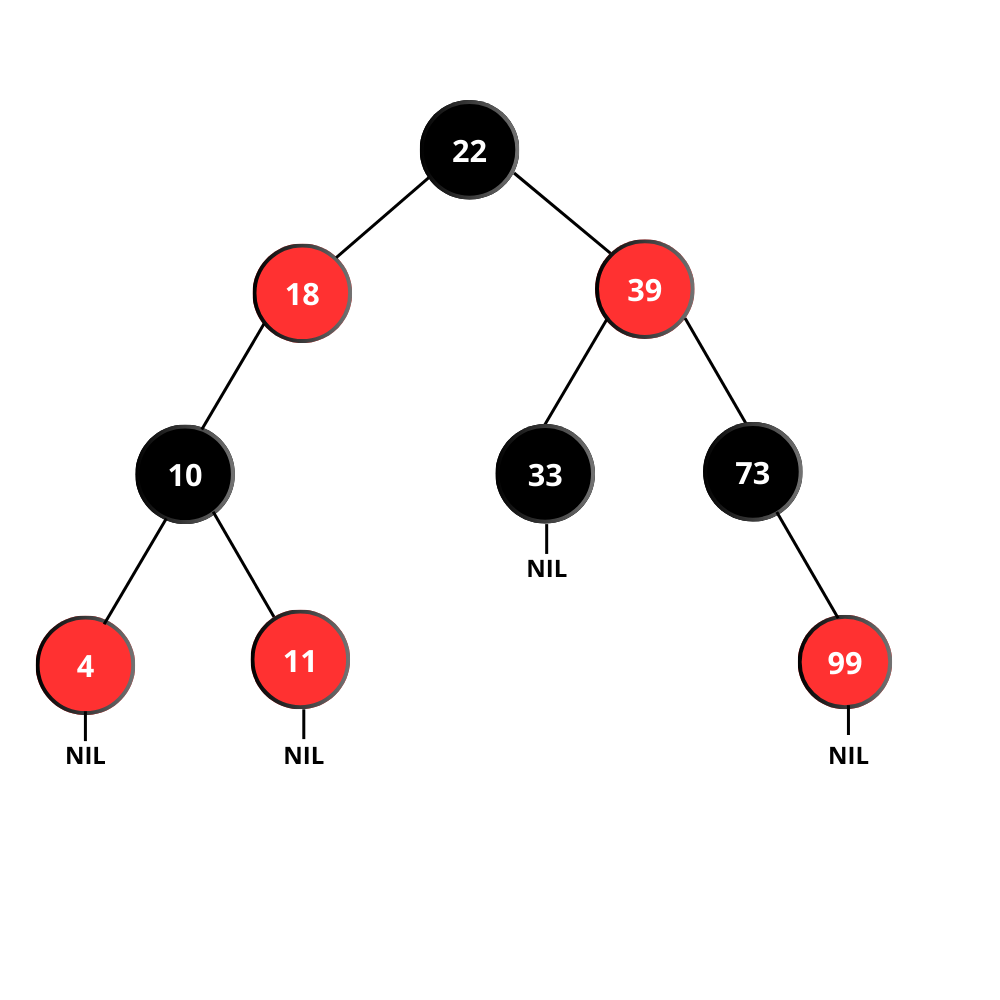
\includegraphics[scale=.32]{RED-BLACK TREE.png}
\end{frame}

\begin{frame}
\frametitle{(1) Waarom een Red-Black tree?}
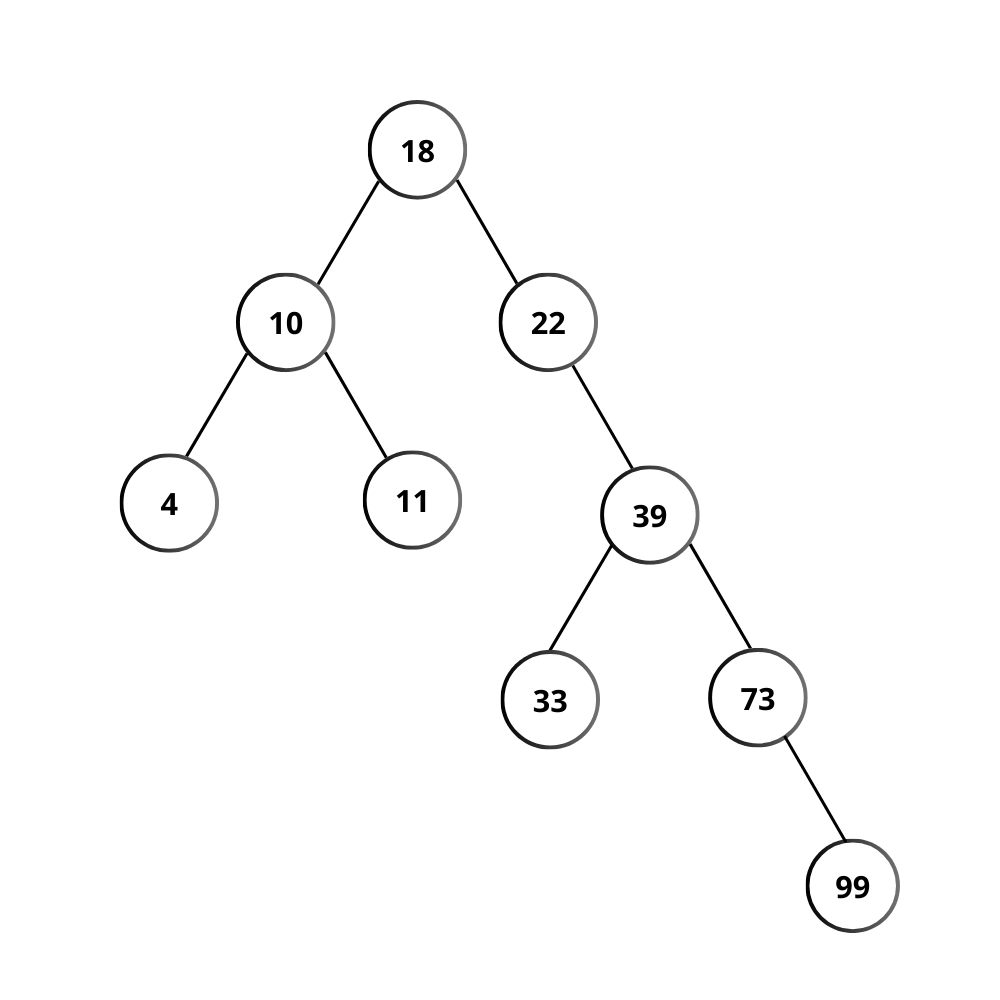
\includegraphics[scale=.3]{3.png}
\end{frame}

\begin{frame}
\frametitle{(1) Waarom een Red-Black tree?}
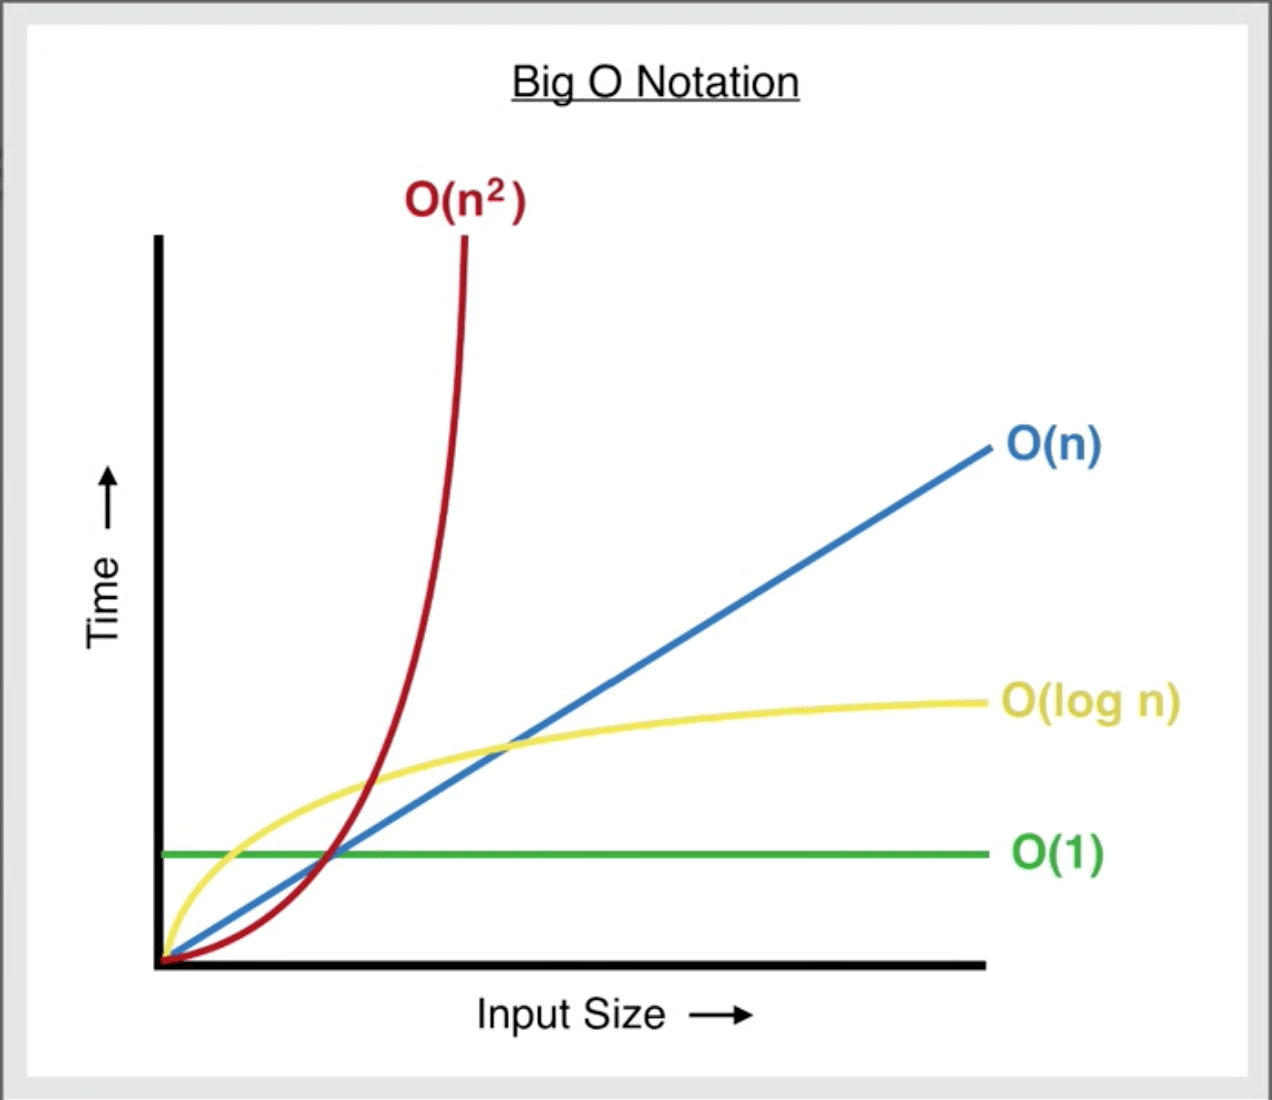
\includegraphics[scale=.18]{time_complexity.png}
\end{frame}

\begin{frame}
\frametitle{(2) Hoe werkt een Red-Black tree?}
Ingebakken regels: \\
\begin{enumerate}
    \item De root is altijd zwart
    \pause
    \item NIL nodes altijd zwart \\
    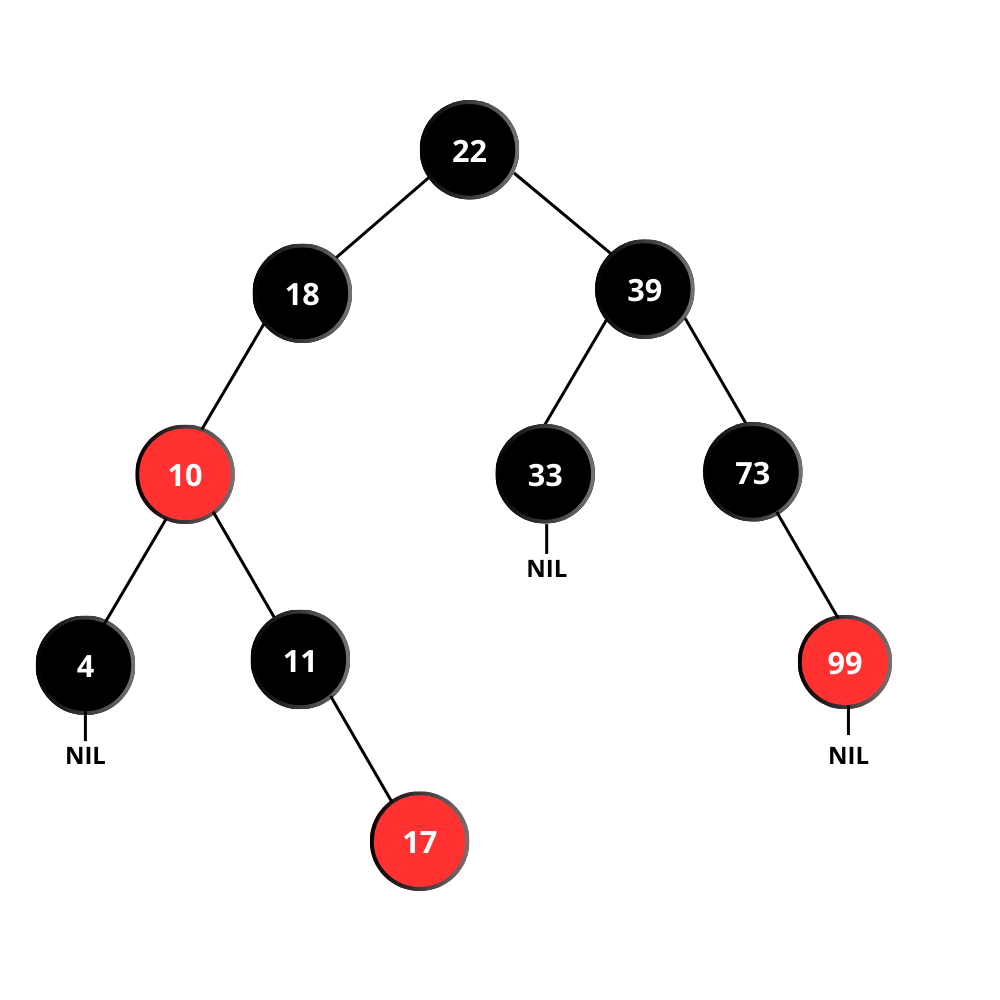
\includegraphics[scale=.20]{DONE.png}
\end{enumerate}
\end{frame}

\begin{frame}
\frametitle{(2) Hoe werkt een Red-Black tree?}
Ingebakken regels: \\
\begin{enumerate}
    \item De root is altijd zwart
    \item NIL nodes altijd zwart
    \item Black height overal gelijk
    \pause
    \item Inserted node is altijd rood
    \pause
    \item Parent en child nooit beide rood
\end{enumerate}
\end{frame}

\begin{frame}
\frametitle{(2) Hoe werkt een Red-Black tree?}
De 4 cases: \\
\begin{enumerate}
    \item De nieuwe node is de root
    \item Parent en Uncle van de nieuwe node zijn rood
    \item Parent van de nieuwe node is zwart (goed)
    \item Parent is rood maar de uncle is black
\end{enumerate}
\end{frame}

\begin{frame}
\frametitle{(3) Voorbeeld van een gebroken case}
    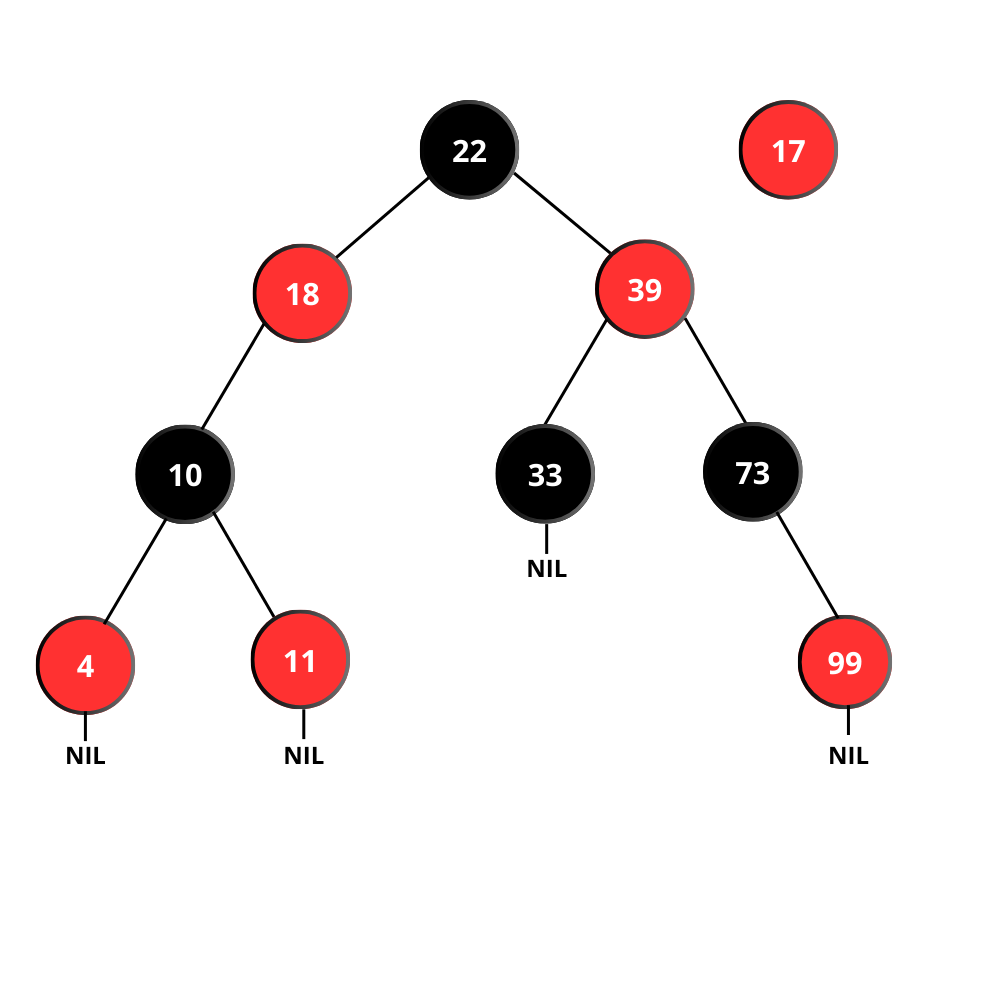
\includegraphics[scale=.30]{PRE-INSERTION.png}
\end{frame}

\begin{frame}
\frametitle{(3) Voorbeeld van een gebroken case}
    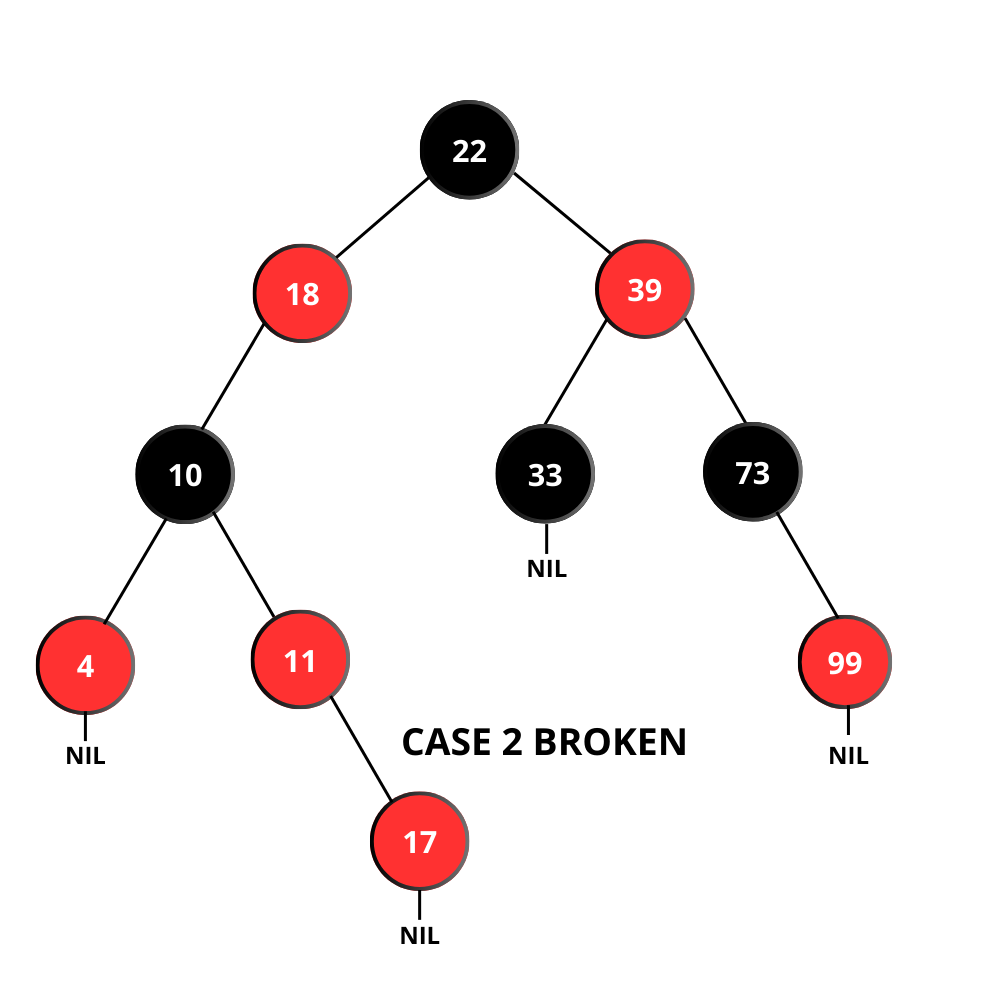
\includegraphics[scale=.30]{CASE2_1.png}
\end{frame}

\begin{frame}
\frametitle{(3) Voorbeeld van een gebroken case}
    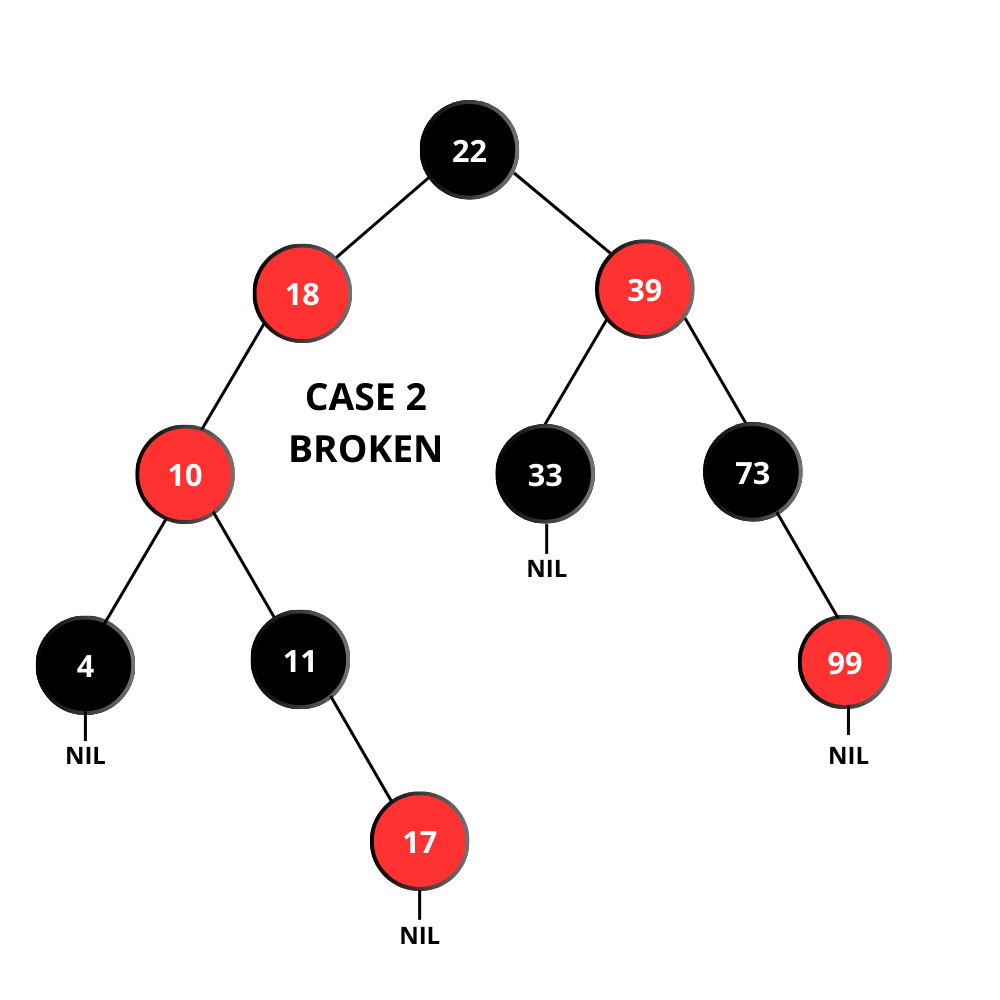
\includegraphics[scale=.30]{CASE2_2.png}
\end{frame}

\begin{frame}
\frametitle{(3) Voorbeeld van een gebroken case}
    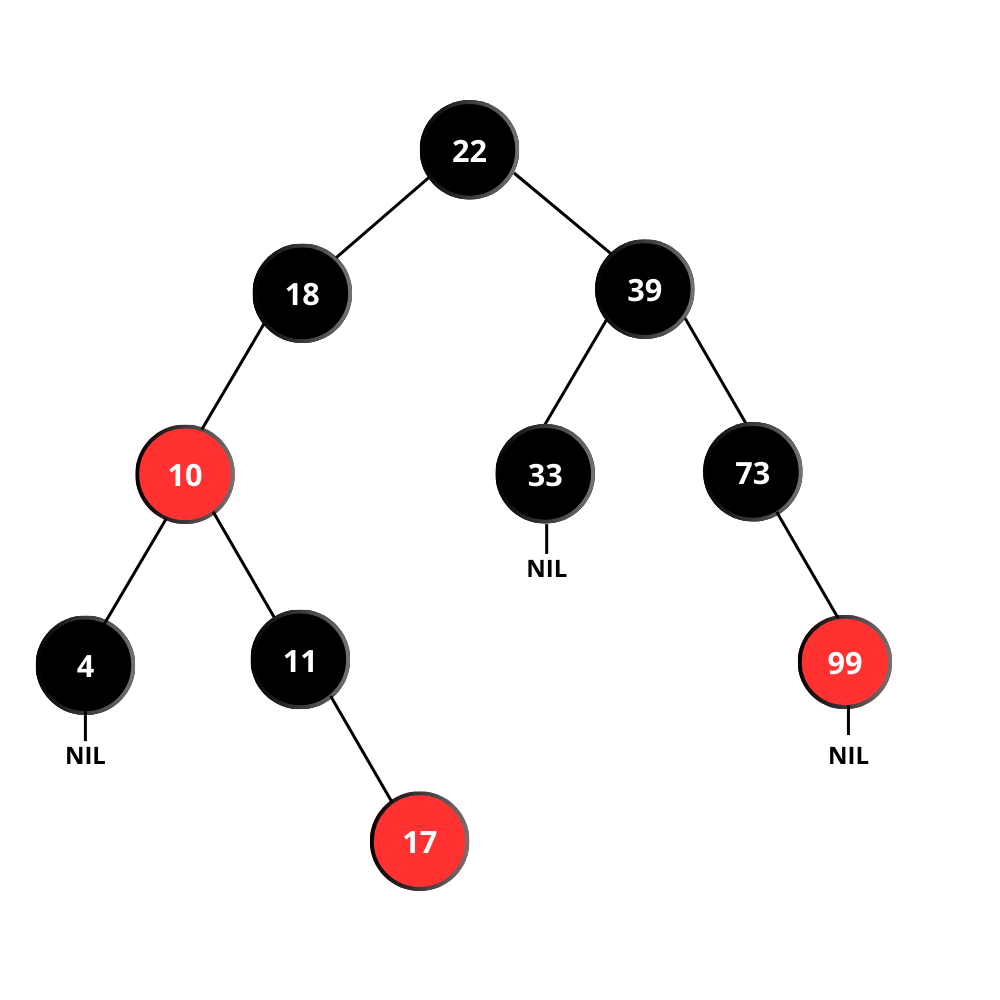
\includegraphics[scale=.30]{DONE.png}
\end{frame}

\begin{frame}
\frametitle{(4) Red-Black tree implementatie}
    Shoutout Boris voor implementatie 
\end{frame}
%-------------------------------------------------------------------------------
\end{document}
